% =====================================================================
% figF1_geometry_law.tex  — R/ggplot2 -> tikzDevice
% Regenerate: Rscript submissions/ieee/figures-src/figF1_geometry_law.R
% Provenance (canonical artifact :: field = plotted value):
% SOURCE: results/C1_mechanism_sc_table.json :: groups[llama1b,rome,cf,L8].within_probe_rho_C = 0.3950
% SOURCE: results/C1_mechanism_sc_table.json :: groups[llama1b,rome,cf,L10].within_probe_rho_C = 0.5337
% SOURCE: results/C1_mechanism_sc_table.json :: groups[llama1b,rome,cf,L12].within_probe_rho_C = 0.6018
% SOURCE: results/C1_mechanism_sc_table.json :: groups[llama1b,rome,cf,L14].within_probe_rho_C = 0.3006
% SOURCE: results/C1_mechanism_sc_table.json :: groups[llama1b,rome,cf,L8].within_probe_rho_SC = 0.4015
% SOURCE: results/C1_mechanism_sc_table.json :: groups[llama1b,rome,cf,L10].within_probe_rho_SC = 0.5526
% SOURCE: results/C1_mechanism_sc_table.json :: groups[llama1b,rome,cf,L12].within_probe_rho_SC = 0.6765
% SOURCE: results/C1_mechanism_sc_table.json :: groups[llama1b,rome,cf,L14].within_probe_rho_SC = 0.5037
% SOURCE: results/G2_gradsim_L8.json :: aggregate.keycos_within_probe.mean = 0.3951
% SOURCE: results/G2_gradsim_L8.json :: aggregate.keycos_within_probe.std = 0.0106
% SOURCE: results/G2_gradsim_L8.json :: aggregate.gradsim_within_probe.normgrowth.mean = 0.4015
% SOURCE: results/G2_gradsim_L8.json :: aggregate.gradsim_within_probe.normgrowth.std = 0.0110
% SOURCE: results/G2_gradsim_L10.json :: aggregate.keycos_within_probe.mean = 0.5337
% SOURCE: results/G2_gradsim_L10.json :: aggregate.keycos_within_probe.std = 0.0105
% SOURCE: results/G2_gradsim_L10.json :: aggregate.gradsim_within_probe.normgrowth.mean = 0.5526
% SOURCE: results/G2_gradsim_L10.json :: aggregate.gradsim_within_probe.normgrowth.std = 0.0107
% SOURCE: results/G2_gradsim_L12.json :: aggregate.keycos_within_probe.mean = 0.6018
% SOURCE: results/G2_gradsim_L12.json :: aggregate.keycos_within_probe.std = 0.0189
% SOURCE: results/G2_gradsim_L12.json :: aggregate.gradsim_within_probe.normgrowth.mean = 0.6765
% SOURCE: results/G2_gradsim_L12.json :: aggregate.gradsim_within_probe.normgrowth.std = 0.0317
% SOURCE: results/G2_gradsim_L14.json :: aggregate.keycos_within_probe.mean = 0.3006
% SOURCE: results/G2_gradsim_L14.json :: aggregate.keycos_within_probe.std = 0.0403
% SOURCE: results/G2_gradsim_L14.json :: aggregate.gradsim_within_probe.normgrowth.mean = 0.5036
% SOURCE: results/G2_gradsim_L14.json :: aggregate.gradsim_within_probe.normgrowth.std = 0.0297
% SOURCE: results/G1_stability_L8_v2.json :: per_seed[gate_llama1b_rome_cf_L8_s0.npz].flat_spearman_INFLATED = 0.4192
% SOURCE: results/G1_stability_L8_v2.json :: per_seed[gate_llama1b_rome_cf_L8_s0.npz].within_probe_mean = 0.4060
% SOURCE: results/G1_stability_L8_v2.json :: per_seed[gate_llama1b_rome_cf_L8_s1.npz].flat_spearman_INFLATED = 0.3886
% SOURCE: results/G1_stability_L8_v2.json :: per_seed[gate_llama1b_rome_cf_L8_s1.npz].within_probe_mean = 0.3984
% SOURCE: results/G1_stability_L8_v2.json :: per_seed[gate_llama1b_rome_cf_L8_s2.npz].flat_spearman_INFLATED = 0.3953
% SOURCE: results/G1_stability_L8_v2.json :: per_seed[gate_llama1b_rome_cf_L8_s2.npz].within_probe_mean = 0.3808
% SOURCE: results/G1_stability_L10_v2.json :: per_seed[gate_llama1b_rome_cf_L10_s0.npz].flat_spearman_INFLATED = 0.5070
% SOURCE: results/G1_stability_L10_v2.json :: per_seed[gate_llama1b_rome_cf_L10_s0.npz].within_probe_mean = 0.5321
% SOURCE: results/G1_stability_L10_v2.json :: per_seed[gate_llama1b_rome_cf_L10_s1.npz].flat_spearman_INFLATED = 0.4476
% SOURCE: results/G1_stability_L10_v2.json :: per_seed[gate_llama1b_rome_cf_L10_s1.npz].within_probe_mean = 0.5218
% SOURCE: results/G1_stability_L10_v2.json :: per_seed[gate_llama1b_rome_cf_L10_s2.npz].flat_spearman_INFLATED = 0.5194
% SOURCE: results/G1_stability_L10_v2.json :: per_seed[gate_llama1b_rome_cf_L10_s2.npz].within_probe_mean = 0.5473
% SOURCE: results/G1_stability_L12_v2.json :: per_seed[gate_llama1b_rome_cf_L12_s0.npz].flat_spearman_INFLATED = 0.5123
% SOURCE: results/G1_stability_L12_v2.json :: per_seed[gate_llama1b_rome_cf_L12_s0.npz].within_probe_mean = 0.6016
% SOURCE: results/G1_stability_L12_v2.json :: per_seed[gate_llama1b_rome_cf_L12_s1.npz].flat_spearman_INFLATED = 0.5269
% SOURCE: results/G1_stability_L12_v2.json :: per_seed[gate_llama1b_rome_cf_L12_s1.npz].within_probe_mean = 0.6250
% SOURCE: results/G1_stability_L12_v2.json :: per_seed[gate_llama1b_rome_cf_L12_s2.npz].flat_spearman_INFLATED = 0.4948
% SOURCE: results/G1_stability_L12_v2.json :: per_seed[gate_llama1b_rome_cf_L12_s2.npz].within_probe_mean = 0.5788
% SOURCE: results/G1_stability_L14_v2.json :: per_seed[gate_llama1b_rome_cf_L14_s0.npz].flat_spearman_INFLATED = 0.2647
% SOURCE: results/G1_stability_L14_v2.json :: per_seed[gate_llama1b_rome_cf_L14_s0.npz].within_probe_mean = 0.2712
% SOURCE: results/G1_stability_L14_v2.json :: per_seed[gate_llama1b_rome_cf_L14_s1.npz].flat_spearman_INFLATED = 0.2643
% SOURCE: results/G1_stability_L14_v2.json :: per_seed[gate_llama1b_rome_cf_L14_s1.npz].within_probe_mean = 0.2731
% SOURCE: results/G1_stability_L14_v2.json :: per_seed[gate_llama1b_rome_cf_L14_s2.npz].flat_spearman_INFLATED = 0.3170
% SOURCE: results/G1_stability_L14_v2.json :: per_seed[gate_llama1b_rome_cf_L14_s2.npz].within_probe_mean = 0.3576
% SOURCE: results/G1_stability_L8_v2.json :: per_seed[gate_llama1b_rome_cf_L8_s0.npz].editlevel_null_mean = -0.0009
% SOURCE: results/G1_stability_L8_v2.json :: per_seed[gate_llama1b_rome_cf_L8_s0.npz].editlevel_null_std = 0.0308
% SOURCE: results/G1_stability_L8_v2.json :: per_seed[gate_llama1b_rome_cf_L8_s0.npz].editlevel_z = 13.2300
% SOURCE: results/G1_stability_L8_v2.json :: per_seed[gate_llama1b_rome_cf_L8_s1.npz].editlevel_null_mean = 0.0015
% SOURCE: results/G1_stability_L8_v2.json :: per_seed[gate_llama1b_rome_cf_L8_s1.npz].editlevel_null_std = 0.0320
% SOURCE: results/G1_stability_L8_v2.json :: per_seed[gate_llama1b_rome_cf_L8_s1.npz].editlevel_z = 12.4100
% SOURCE: results/G1_stability_L8_v2.json :: per_seed[gate_llama1b_rome_cf_L8_s2.npz].editlevel_null_mean = -0.0002
% SOURCE: results/G1_stability_L8_v2.json :: per_seed[gate_llama1b_rome_cf_L8_s2.npz].editlevel_null_std = 0.0312
% SOURCE: results/G1_stability_L8_v2.json :: per_seed[gate_llama1b_rome_cf_L8_s2.npz].editlevel_z = 12.2300
% SOURCE: results/G1_stability_L10_v2.json :: per_seed[gate_llama1b_rome_cf_L10_s0.npz].editlevel_null_mean = -0.0005
% SOURCE: results/G1_stability_L10_v2.json :: per_seed[gate_llama1b_rome_cf_L10_s0.npz].editlevel_null_std = 0.0343
% SOURCE: results/G1_stability_L10_v2.json :: per_seed[gate_llama1b_rome_cf_L10_s0.npz].editlevel_z = 15.5400
% SOURCE: results/G1_stability_L10_v2.json :: per_seed[gate_llama1b_rome_cf_L10_s1.npz].editlevel_null_mean = 0.0017
% SOURCE: results/G1_stability_L10_v2.json :: per_seed[gate_llama1b_rome_cf_L10_s1.npz].editlevel_null_std = 0.0341
% SOURCE: results/G1_stability_L10_v2.json :: per_seed[gate_llama1b_rome_cf_L10_s1.npz].editlevel_z = 15.2400
% SOURCE: results/G1_stability_L10_v2.json :: per_seed[gate_llama1b_rome_cf_L10_s2.npz].editlevel_null_mean = -0.0004
% SOURCE: results/G1_stability_L10_v2.json :: per_seed[gate_llama1b_rome_cf_L10_s2.npz].editlevel_null_std = 0.0335
% SOURCE: results/G1_stability_L10_v2.json :: per_seed[gate_llama1b_rome_cf_L10_s2.npz].editlevel_z = 16.3600
% SOURCE: results/G1_stability_L12_v2.json :: per_seed[gate_llama1b_rome_cf_L12_s0.npz].editlevel_null_mean = -0.0005
% SOURCE: results/G1_stability_L12_v2.json :: per_seed[gate_llama1b_rome_cf_L12_s0.npz].editlevel_null_std = 0.0453
% SOURCE: results/G1_stability_L12_v2.json :: per_seed[gate_llama1b_rome_cf_L12_s0.npz].editlevel_z = 13.2800
% SOURCE: results/G1_stability_L12_v2.json :: per_seed[gate_llama1b_rome_cf_L12_s1.npz].editlevel_null_mean = 0.0013
% SOURCE: results/G1_stability_L12_v2.json :: per_seed[gate_llama1b_rome_cf_L12_s1.npz].editlevel_null_std = 0.0455
% SOURCE: results/G1_stability_L12_v2.json :: per_seed[gate_llama1b_rome_cf_L12_s1.npz].editlevel_z = 13.6900
% SOURCE: results/G1_stability_L12_v2.json :: per_seed[gate_llama1b_rome_cf_L12_s2.npz].editlevel_null_mean = -0.0026
% SOURCE: results/G1_stability_L12_v2.json :: per_seed[gate_llama1b_rome_cf_L12_s2.npz].editlevel_null_std = 0.0452
% SOURCE: results/G1_stability_L12_v2.json :: per_seed[gate_llama1b_rome_cf_L12_s2.npz].editlevel_z = 12.8600
% SOURCE: results/G1_stability_L14_v2.json :: per_seed[gate_llama1b_rome_cf_L14_s0.npz].editlevel_null_mean = 0.0007
% SOURCE: results/G1_stability_L14_v2.json :: per_seed[gate_llama1b_rome_cf_L14_s0.npz].editlevel_null_std = 0.0399
% SOURCE: results/G1_stability_L14_v2.json :: per_seed[gate_llama1b_rome_cf_L14_s0.npz].editlevel_z = 6.7800
% SOURCE: results/G1_stability_L14_v2.json :: per_seed[gate_llama1b_rome_cf_L14_s1.npz].editlevel_null_mean = -0.0008
% SOURCE: results/G1_stability_L14_v2.json :: per_seed[gate_llama1b_rome_cf_L14_s1.npz].editlevel_null_std = 0.0419
% SOURCE: results/G1_stability_L14_v2.json :: per_seed[gate_llama1b_rome_cf_L14_s1.npz].editlevel_z = 6.5400
% SOURCE: results/G1_stability_L14_v2.json :: per_seed[gate_llama1b_rome_cf_L14_s2.npz].editlevel_null_mean = -0.0006
% SOURCE: results/G1_stability_L14_v2.json :: per_seed[gate_llama1b_rome_cf_L14_s2.npz].editlevel_null_std = 0.0422
% SOURCE: results/G1_stability_L14_v2.json :: per_seed[gate_llama1b_rome_cf_L14_s2.npz].editlevel_z = 8.4900
% SOURCE: results/G1_stability_L8_v2.json :: aggregate.max_within_probe_perm_p_editlevel = 0.0010
% SOURCE: results/G1_stability_L10_v2.json :: aggregate.max_within_probe_perm_p_editlevel = 0.0010
% SOURCE: results/G1_stability_L12_v2.json :: aggregate.max_within_probe_perm_p_editlevel = 0.0010
% SOURCE: results/G1_stability_L14_v2.json :: aggregate.max_within_probe_perm_p_editlevel = 0.0010
% =====================================================================
% !TEX encoding = UTF-8 Unicode
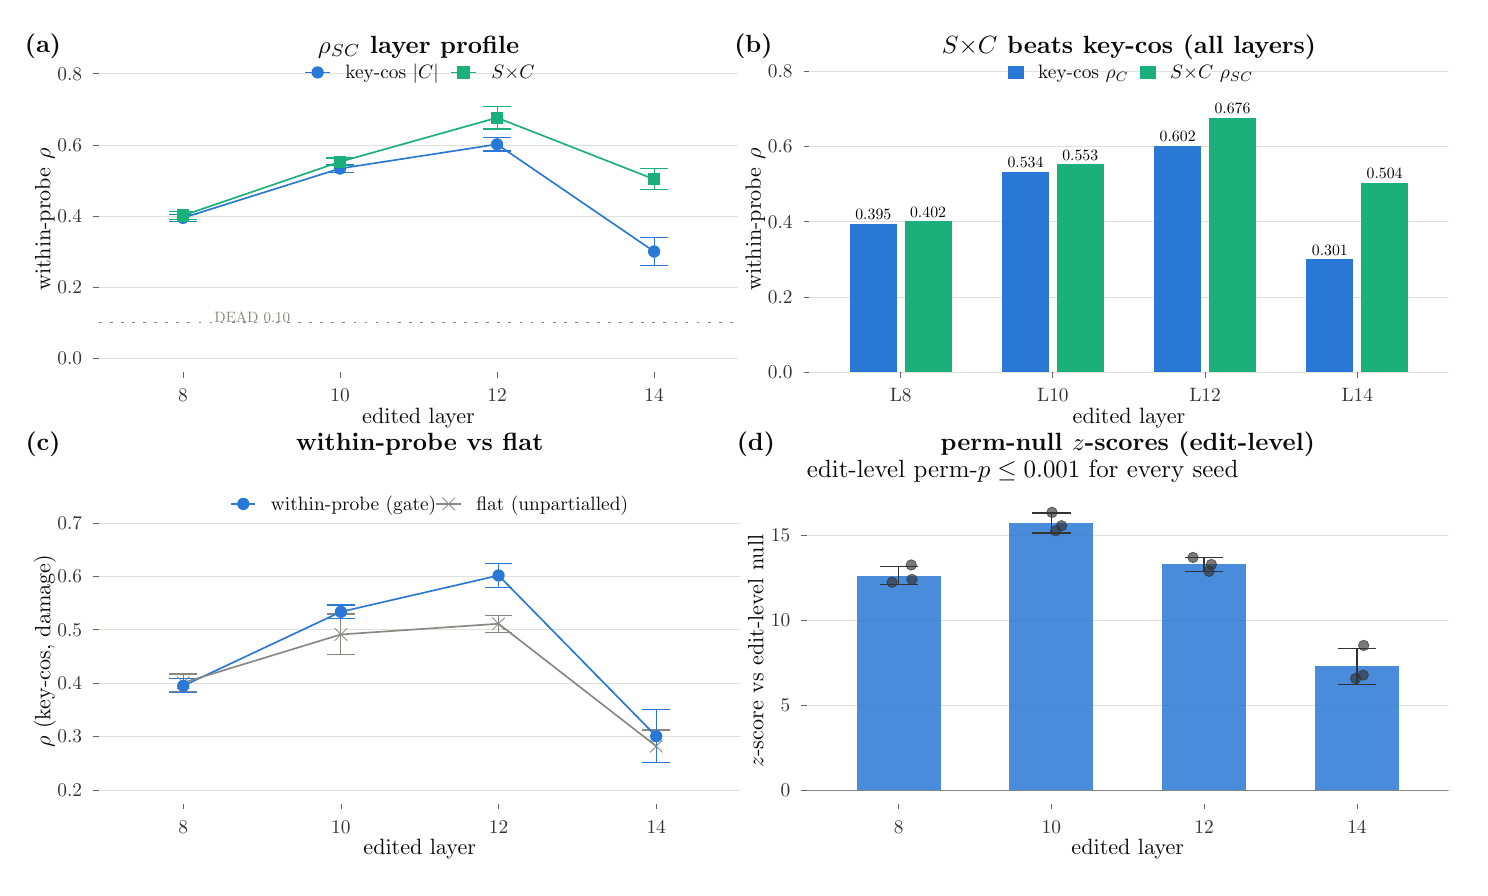
\begin{tikzpicture}[x=1pt,y=1pt]
\definecolor{fillColor}{RGB}{255,255,255}
\path[use as bounding box,fill=fillColor,fill opacity=0.00] (0,0) rectangle (517.45,303.53);
\begin{scope}
\path[clip] (  0.00,  0.00) rectangle (517.45,303.53);
\definecolor{drawColor}{RGB}{255,255,255}
\definecolor{fillColor}{RGB}{255,255,255}

\path[draw=drawColor,line width= 0.6pt,line join=round,line cap=round,fill=fillColor] (  0.00,  0.00) rectangle (517.45,303.53);
\end{scope}
\begin{scope}
\path[clip] (  2.00,157.92) rectangle (258.73,301.53);
\definecolor{fillColor}{RGB}{255,255,255}

\path[fill=fillColor] (  2.00,157.92) rectangle (258.73,301.53);
\end{scope}
\begin{scope}
\path[clip] (258.73,157.92) rectangle (515.45,301.53);
\definecolor{fillColor}{RGB}{255,255,255}

\path[fill=fillColor] (258.73,157.92) rectangle (515.45,301.53);
\end{scope}
\begin{scope}
\path[clip] ( 25.74,178.98) rectangle (256.73,289.31);
\definecolor{drawColor}{RGB}{225,224,217}

\path[draw=drawColor,line width= 0.3pt,line join=round] ( 25.74,184.00) --
	(256.73,184.00);

\path[draw=drawColor,line width= 0.3pt,line join=round] ( 25.74,209.72) --
	(256.73,209.72);

\path[draw=drawColor,line width= 0.3pt,line join=round] ( 25.74,235.43) --
	(256.73,235.43);

\path[draw=drawColor,line width= 0.3pt,line join=round] ( 25.74,261.15) --
	(256.73,261.15);

\path[draw=drawColor,line width= 0.3pt,line join=round] ( 25.74,286.87) --
	(256.73,286.87);
\definecolor{drawColor}{RGB}{137,135,129}

\path[draw=drawColor,line width= 0.3pt,dash pattern=on 1pt off 3pt ,line join=round] ( 25.74,196.86) -- (256.73,196.86);

\node[text=drawColor,anchor=base west,inner sep=0pt, outer sep=0pt, scale=  0.54] at ( 67.45,197.03) {DEAD 0.10};
\definecolor{drawColor}{RGB}{42,120,214}

\path[draw=drawColor,line width= 0.4pt,line join=round] ( 51.14,236.17) --
	( 61.07,236.17);

\path[draw=drawColor,line width= 0.4pt,line join=round] ( 56.10,236.17) --
	( 56.10,233.44);

\path[draw=drawColor,line width= 0.4pt,line join=round] ( 51.14,233.44) --
	( 61.07,233.44);

\path[draw=drawColor,line width= 0.4pt,line join=round] (107.89,253.98) --
	(117.82,253.98);

\path[draw=drawColor,line width= 0.4pt,line join=round] (112.86,253.98) --
	(112.86,251.28);

\path[draw=drawColor,line width= 0.4pt,line join=round] (107.89,251.28) --
	(117.82,251.28);

\path[draw=drawColor,line width= 0.4pt,line join=round] (164.64,263.81) --
	(174.58,263.81);

\path[draw=drawColor,line width= 0.4pt,line join=round] (169.61,263.81) --
	(169.61,258.95);

\path[draw=drawColor,line width= 0.4pt,line join=round] (164.64,258.95) --
	(174.58,258.95);

\path[draw=drawColor,line width= 0.4pt,line join=round] (221.40,227.83) --
	(231.33,227.83);

\path[draw=drawColor,line width= 0.4pt,line join=round] (226.36,227.83) --
	(226.36,217.47);

\path[draw=drawColor,line width= 0.4pt,line join=round] (221.40,217.47) --
	(231.33,217.47);
\definecolor{drawColor}{RGB}{27,175,122}

\path[draw=drawColor,line width= 0.4pt,line join=round] ( 51.14,237.04) --
	( 61.07,237.04);

\path[draw=drawColor,line width= 0.4pt,line join=round] ( 56.10,237.04) --
	( 56.10,234.21);

\path[draw=drawColor,line width= 0.4pt,line join=round] ( 51.14,234.21) --
	( 61.07,234.21);

\path[draw=drawColor,line width= 0.4pt,line join=round] (107.89,256.43) --
	(117.82,256.43);

\path[draw=drawColor,line width= 0.4pt,line join=round] (112.86,256.43) --
	(112.86,253.68);

\path[draw=drawColor,line width= 0.4pt,line join=round] (107.89,253.68) --
	(117.82,253.68);

\path[draw=drawColor,line width= 0.4pt,line join=round] (164.64,275.06) --
	(174.58,275.06);

\path[draw=drawColor,line width= 0.4pt,line join=round] (169.61,275.06) --
	(169.61,266.91);

\path[draw=drawColor,line width= 0.4pt,line join=round] (164.64,266.91) --
	(174.58,266.91);

\path[draw=drawColor,line width= 0.4pt,line join=round] (221.40,252.57) --
	(231.33,252.57);

\path[draw=drawColor,line width= 0.4pt,line join=round] (226.36,252.57) --
	(226.36,244.94);

\path[draw=drawColor,line width= 0.4pt,line join=round] (221.40,244.94) --
	(231.33,244.94);
\definecolor{drawColor}{RGB}{42,120,214}

\path[draw=drawColor,line width= 0.6pt,line join=round] ( 56.10,234.80) --
	(112.86,252.63) --
	(169.61,261.38) --
	(226.36,222.65);
\definecolor{drawColor}{RGB}{27,175,122}

\path[draw=drawColor,line width= 0.6pt,line join=round] ( 56.10,235.63) --
	(112.86,255.06) --
	(169.61,270.99) --
	(226.36,248.76);
\definecolor{fillColor}{RGB}{42,120,214}

\path[fill=fillColor] ( 56.10,234.80) circle (  2.22);

\path[fill=fillColor] (112.86,252.63) circle (  2.22);

\path[fill=fillColor] (169.61,261.38) circle (  2.22);

\path[fill=fillColor] (226.36,222.65) circle (  2.22);
\definecolor{fillColor}{RGB}{27,175,122}

\path[fill=fillColor] ( 53.88,233.41) --
	( 58.32,233.41) --
	( 58.32,237.85) --
	( 53.88,237.85) --
	cycle;

\path[fill=fillColor] (110.64,252.84) --
	(115.08,252.84) --
	(115.08,257.27) --
	(110.64,257.27) --
	cycle;

\path[fill=fillColor] (167.39,268.77) --
	(171.83,268.77) --
	(171.83,273.21) --
	(167.39,273.21) --
	cycle;

\path[fill=fillColor] (224.14,246.54) --
	(228.58,246.54) --
	(228.58,250.97) --
	(224.14,250.97) --
	cycle;
\end{scope}
\begin{scope}
\path[clip] (  0.00,  0.00) rectangle (517.45,303.53);
\definecolor{drawColor}{gray}{0.20}

\node[text=drawColor,anchor=base east,inner sep=0pt, outer sep=0pt, scale=  0.70] at ( 19.69,181.72) {0.0};

\node[text=drawColor,anchor=base east,inner sep=0pt, outer sep=0pt, scale=  0.70] at ( 19.69,207.44) {0.2};

\node[text=drawColor,anchor=base east,inner sep=0pt, outer sep=0pt, scale=  0.70] at ( 19.69,233.16) {0.4};

\node[text=drawColor,anchor=base east,inner sep=0pt, outer sep=0pt, scale=  0.70] at ( 19.69,258.87) {0.6};

\node[text=drawColor,anchor=base east,inner sep=0pt, outer sep=0pt, scale=  0.70] at ( 19.69,284.59) {0.8};
\end{scope}
\begin{scope}
\path[clip] (  0.00,  0.00) rectangle (517.45,303.53);
\definecolor{drawColor}{gray}{0.40}

\path[draw=drawColor,line width= 0.3pt,line join=round] ( 23.74,184.00) --
	( 25.74,184.00);

\path[draw=drawColor,line width= 0.3pt,line join=round] ( 23.74,209.72) --
	( 25.74,209.72);

\path[draw=drawColor,line width= 0.3pt,line join=round] ( 23.74,235.43) --
	( 25.74,235.43);

\path[draw=drawColor,line width= 0.3pt,line join=round] ( 23.74,261.15) --
	( 25.74,261.15);

\path[draw=drawColor,line width= 0.3pt,line join=round] ( 23.74,286.87) --
	( 25.74,286.87);
\end{scope}
\begin{scope}
\path[clip] (  0.00,  0.00) rectangle (517.45,303.53);
\definecolor{drawColor}{gray}{0.40}

\path[draw=drawColor,line width= 0.3pt,line join=round] ( 56.10,176.98) --
	( 56.10,178.98);

\path[draw=drawColor,line width= 0.3pt,line join=round] (112.86,176.98) --
	(112.86,178.98);

\path[draw=drawColor,line width= 0.3pt,line join=round] (169.61,176.98) --
	(169.61,178.98);

\path[draw=drawColor,line width= 0.3pt,line join=round] (226.36,176.98) --
	(226.36,178.98);
\end{scope}
\begin{scope}
\path[clip] (  0.00,  0.00) rectangle (517.45,303.53);
\definecolor{drawColor}{gray}{0.20}

\node[text=drawColor,anchor=base,inner sep=0pt, outer sep=0pt, scale=  0.70] at ( 56.10,168.38) {8};

\node[text=drawColor,anchor=base,inner sep=0pt, outer sep=0pt, scale=  0.70] at (112.86,168.38) {10};

\node[text=drawColor,anchor=base,inner sep=0pt, outer sep=0pt, scale=  0.70] at (169.61,168.38) {12};

\node[text=drawColor,anchor=base,inner sep=0pt, outer sep=0pt, scale=  0.70] at (226.36,168.38) {14};
\end{scope}
\begin{scope}
\path[clip] (  0.00,  0.00) rectangle (517.45,303.53);
\definecolor{drawColor}{RGB}{11,11,11}

\node[text=drawColor,anchor=base,inner sep=0pt, outer sep=0pt, scale=  0.80] at (141.23,160.65) {edited layer};
\end{scope}
\begin{scope}
\path[clip] (  0.00,  0.00) rectangle (517.45,303.53);
\definecolor{drawColor}{RGB}{11,11,11}

\node[text=drawColor,rotate= 90.00,anchor=base,inner sep=0pt, outer sep=0pt, scale=  0.80] at (  8.21,234.15) {within-probe $\rho$};
\end{scope}
\begin{scope}
\path[clip] (  0.00,  0.00) rectangle (517.45,303.53);
\definecolor{drawColor}{RGB}{42,120,214}

\path[draw=drawColor,line width= 0.4pt,line join=round] (100.39,287.35) -- (109.19,287.35);

\path[draw=drawColor,line width= 0.6pt,line join=round] (100.39,287.35) -- (109.19,287.35);
\definecolor{fillColor}{RGB}{42,120,214}

\path[fill=fillColor] (104.79,287.35) circle (  2.22);
\end{scope}
\begin{scope}
\path[clip] (  0.00,  0.00) rectangle (517.45,303.53);
\definecolor{drawColor}{RGB}{27,175,122}

\path[draw=drawColor,line width= 0.4pt,line join=round] (153.13,287.35) -- (161.93,287.35);

\path[draw=drawColor,line width= 0.6pt,line join=round] (153.13,287.35) -- (161.93,287.35);
\definecolor{fillColor}{RGB}{27,175,122}

\path[fill=fillColor] (155.31,285.13) --
	(159.75,285.13) --
	(159.75,289.57) --
	(155.31,289.57) --
	cycle;
\end{scope}
\begin{scope}
\path[clip] (  0.00,  0.00) rectangle (517.45,303.53);
\definecolor{drawColor}{RGB}{11,11,11}

\node[text=drawColor,anchor=base west,inner sep=0pt, outer sep=0pt, scale=  0.70] at (114.79,285.07) {key-cos $|C|$};
\end{scope}
\begin{scope}
\path[clip] (  0.00,  0.00) rectangle (517.45,303.53);
\definecolor{drawColor}{RGB}{11,11,11}

\node[text=drawColor,anchor=base west,inner sep=0pt, outer sep=0pt, scale=  0.70] at (167.53,285.07) {$S{\times}C$};
\end{scope}
\begin{scope}
\path[clip] (  0.00,  0.00) rectangle (517.45,303.53);
\definecolor{drawColor}{RGB}{11,11,11}

\node[text=drawColor,anchor=base,inner sep=0pt, outer sep=0pt, scale=  0.90] at (141.23,294.33) {\bfseries $\rho_{SC}$ layer profile};
\end{scope}
\begin{scope}
\path[clip] (  0.00,  0.00) rectangle (517.45,303.53);
\definecolor{drawColor}{RGB}{11,11,11}

\node[text=drawColor,anchor=base,inner sep=0pt, outer sep=0pt, scale=  0.90] at (  5.54,294.60) {\bfseries (a)};
\end{scope}
\begin{scope}
\path[clip] (282.47,178.98) rectangle (513.45,289.31);
\definecolor{drawColor}{RGB}{225,224,217}

\path[draw=drawColor,line width= 0.3pt,line join=round] (282.47,178.98) --
	(513.45,178.98);

\path[draw=drawColor,line width= 0.3pt,line join=round] (282.47,206.16) --
	(513.45,206.16);

\path[draw=drawColor,line width= 0.3pt,line join=round] (282.47,233.35) --
	(513.45,233.35);

\path[draw=drawColor,line width= 0.3pt,line join=round] (282.47,260.53) --
	(513.45,260.53);

\path[draw=drawColor,line width= 0.3pt,line join=round] (282.47,287.71) --
	(513.45,287.71);
\definecolor{fillColor}{RGB}{42,120,214}

\path[fill=fillColor] (297.04,178.98) rectangle (314.09,232.67);

\path[fill=fillColor] (352.04,178.98) rectangle (369.09,251.52);

\path[fill=fillColor] (407.03,178.98) rectangle (424.08,260.77);

\path[fill=fillColor] (462.03,178.98) rectangle (479.08,219.84);
\definecolor{fillColor}{RGB}{27,175,122}

\path[fill=fillColor] (316.84,178.98) rectangle (333.89,233.55);

\path[fill=fillColor] (371.84,178.98) rectangle (388.89,254.09);

\path[fill=fillColor] (426.83,178.98) rectangle (443.88,270.92);

\path[fill=fillColor] (481.83,178.98) rectangle (498.88,247.44);
\definecolor{drawColor}{RGB}{0,0,0}

\node[text=drawColor,anchor=base,inner sep=0pt, outer sep=0pt, scale=  0.57] at (305.57,234.15) {0.395};

\node[text=drawColor,anchor=base,inner sep=0pt, outer sep=0pt, scale=  0.57] at (360.56,253.00) {0.534};

\node[text=drawColor,anchor=base,inner sep=0pt, outer sep=0pt, scale=  0.57] at (415.56,262.25) {0.602};

\node[text=drawColor,anchor=base,inner sep=0pt, outer sep=0pt, scale=  0.57] at (470.56,221.32) {0.301};

\node[text=drawColor,anchor=base,inner sep=0pt, outer sep=0pt, scale=  0.57] at (325.36,235.03) {0.402};

\node[text=drawColor,anchor=base,inner sep=0pt, outer sep=0pt, scale=  0.57] at (380.36,255.57) {0.553};

\node[text=drawColor,anchor=base,inner sep=0pt, outer sep=0pt, scale=  0.57] at (435.36,272.41) {0.676};

\node[text=drawColor,anchor=base,inner sep=0pt, outer sep=0pt, scale=  0.57] at (490.35,248.92) {0.504};
\end{scope}
\begin{scope}
\path[clip] (  0.00,  0.00) rectangle (517.45,303.53);
\definecolor{drawColor}{gray}{0.20}

\node[text=drawColor,anchor=base east,inner sep=0pt, outer sep=0pt, scale=  0.70] at (276.42,176.70) {0.0};

\node[text=drawColor,anchor=base east,inner sep=0pt, outer sep=0pt, scale=  0.70] at (276.42,203.89) {0.2};

\node[text=drawColor,anchor=base east,inner sep=0pt, outer sep=0pt, scale=  0.70] at (276.42,231.07) {0.4};

\node[text=drawColor,anchor=base east,inner sep=0pt, outer sep=0pt, scale=  0.70] at (276.42,258.25) {0.6};

\node[text=drawColor,anchor=base east,inner sep=0pt, outer sep=0pt, scale=  0.70] at (276.42,285.43) {0.8};
\end{scope}
\begin{scope}
\path[clip] (  0.00,  0.00) rectangle (517.45,303.53);
\definecolor{drawColor}{gray}{0.40}

\path[draw=drawColor,line width= 0.3pt,line join=round] (280.47,178.98) --
	(282.47,178.98);

\path[draw=drawColor,line width= 0.3pt,line join=round] (280.47,206.16) --
	(282.47,206.16);

\path[draw=drawColor,line width= 0.3pt,line join=round] (280.47,233.35) --
	(282.47,233.35);

\path[draw=drawColor,line width= 0.3pt,line join=round] (280.47,260.53) --
	(282.47,260.53);

\path[draw=drawColor,line width= 0.3pt,line join=round] (280.47,287.71) --
	(282.47,287.71);
\end{scope}
\begin{scope}
\path[clip] (  0.00,  0.00) rectangle (517.45,303.53);
\definecolor{drawColor}{gray}{0.40}

\path[draw=drawColor,line width= 0.3pt,line join=round] (315.46,176.98) --
	(315.46,178.98);

\path[draw=drawColor,line width= 0.3pt,line join=round] (370.46,176.98) --
	(370.46,178.98);

\path[draw=drawColor,line width= 0.3pt,line join=round] (425.46,176.98) --
	(425.46,178.98);

\path[draw=drawColor,line width= 0.3pt,line join=round] (480.46,176.98) --
	(480.46,178.98);
\end{scope}
\begin{scope}
\path[clip] (  0.00,  0.00) rectangle (517.45,303.53);
\definecolor{drawColor}{gray}{0.20}

\node[text=drawColor,anchor=base,inner sep=0pt, outer sep=0pt, scale=  0.70] at (315.46,168.38) {L8};

\node[text=drawColor,anchor=base,inner sep=0pt, outer sep=0pt, scale=  0.70] at (370.46,168.38) {L10};

\node[text=drawColor,anchor=base,inner sep=0pt, outer sep=0pt, scale=  0.70] at (425.46,168.38) {L12};

\node[text=drawColor,anchor=base,inner sep=0pt, outer sep=0pt, scale=  0.70] at (480.46,168.38) {L14};
\end{scope}
\begin{scope}
\path[clip] (  0.00,  0.00) rectangle (517.45,303.53);
\definecolor{drawColor}{RGB}{11,11,11}

\node[text=drawColor,anchor=base,inner sep=0pt, outer sep=0pt, scale=  0.80] at (397.96,160.65) {edited layer};
\end{scope}
\begin{scope}
\path[clip] (  0.00,  0.00) rectangle (517.45,303.53);
\definecolor{drawColor}{RGB}{11,11,11}

\node[text=drawColor,rotate= 90.00,anchor=base,inner sep=0pt, outer sep=0pt, scale=  0.80] at (264.93,234.15) {within-probe $\rho$};
\end{scope}
\begin{scope}
\path[clip] (  0.00,  0.00) rectangle (517.45,303.53);
\definecolor{fillColor}{RGB}{42,120,214}

\path[fill=fillColor] (354.24,284.89) rectangle (360.08,289.80);
\end{scope}
\begin{scope}
\path[clip] (  0.00,  0.00) rectangle (517.45,303.53);
\definecolor{fillColor}{RGB}{27,175,122}

\path[fill=fillColor] (401.91,284.89) rectangle (407.75,289.80);
\end{scope}
\begin{scope}
\path[clip] (  0.00,  0.00) rectangle (517.45,303.53);
\definecolor{drawColor}{RGB}{11,11,11}

\node[text=drawColor,anchor=base west,inner sep=0pt, outer sep=0pt, scale=  0.70] at (365.16,285.07) {key-cos $\rho_C$};
\end{scope}
\begin{scope}
\path[clip] (  0.00,  0.00) rectangle (517.45,303.53);
\definecolor{drawColor}{RGB}{11,11,11}

\node[text=drawColor,anchor=base west,inner sep=0pt, outer sep=0pt, scale=  0.70] at (412.83,285.07) {$S{\times}C$ $\rho_{SC}$};
\end{scope}
\begin{scope}
\path[clip] (  0.00,  0.00) rectangle (517.45,303.53);
\definecolor{drawColor}{RGB}{11,11,11}

\node[text=drawColor,anchor=base,inner sep=0pt, outer sep=0pt, scale=  0.90] at (397.96,294.33) {\bfseries $S{\times}C$ beats key-cos (all layers)};
\end{scope}
\begin{scope}
\path[clip] (  0.00,  0.00) rectangle (517.45,303.53);
\definecolor{drawColor}{RGB}{11,11,11}

\node[text=drawColor,anchor=base,inner sep=0pt, outer sep=0pt, scale=  0.90] at (262.26,294.60) {\bfseries (b)};
\end{scope}
\begin{scope}
\path[clip] (  2.00,  2.00) rectangle (259.60,157.92);
\definecolor{fillColor}{RGB}{255,255,255}

\path[fill=fillColor] (  2.00,  2.00) rectangle (259.60,157.92);
\end{scope}
\begin{scope}
\path[clip] (259.60,  2.00) rectangle (515.45,157.92);
\definecolor{fillColor}{RGB}{255,255,255}

\path[fill=fillColor] (259.60,  2.00) rectangle (515.45,157.92);
\end{scope}
\begin{scope}
\path[clip] ( 25.74, 23.06) rectangle (257.60,133.39);
\definecolor{drawColor}{RGB}{225,224,217}

\path[draw=drawColor,line width= 0.3pt,line join=round] ( 25.74, 28.08) --
	(257.60, 28.08);

\path[draw=drawColor,line width= 0.3pt,line join=round] ( 25.74, 47.37) --
	(257.60, 47.37);

\path[draw=drawColor,line width= 0.3pt,line join=round] ( 25.74, 66.65) --
	(257.60, 66.65);

\path[draw=drawColor,line width= 0.3pt,line join=round] ( 25.74, 85.94) --
	(257.60, 85.94);

\path[draw=drawColor,line width= 0.3pt,line join=round] ( 25.74,105.23) --
	(257.60,105.23);

\path[draw=drawColor,line width= 0.3pt,line join=round] ( 25.74,124.52) --
	(257.60,124.52);
\definecolor{drawColor}{RGB}{137,135,129}

\path[draw=drawColor,line width= 0.3pt,dash pattern=on 1pt off 3pt ,line join=round] ( 25.74,  8.79) -- (257.60,  8.79);

\node[text=drawColor,anchor=base west,inner sep=0pt, outer sep=0pt, scale=  0.54] at ( 67.61,  9.92) {DEAD 0.10};

\path[draw=drawColor,line width= 0.4pt,line join=round] ( 51.23, 69.96) --
	( 61.20, 69.96);

\path[draw=drawColor,line width= 0.4pt,line join=round] ( 56.22, 69.96) --
	( 56.22, 63.75);

\path[draw=drawColor,line width= 0.4pt,line join=round] ( 51.23, 63.75) --
	( 61.20, 63.75);

\path[draw=drawColor,line width= 0.4pt,line join=round] (108.20, 91.67) --
	(118.17, 91.67);

\path[draw=drawColor,line width= 0.4pt,line join=round] (113.19, 91.67) --
	(113.19, 76.87);

\path[draw=drawColor,line width= 0.4pt,line join=round] (108.20, 76.87) --
	(118.17, 76.87);

\path[draw=drawColor,line width= 0.4pt,line join=round] (165.17, 91.23) --
	(175.14, 91.23);

\path[draw=drawColor,line width= 0.4pt,line join=round] (170.15, 91.23) --
	(170.15, 85.03);

\path[draw=drawColor,line width= 0.4pt,line join=round] (165.17, 85.03) --
	(175.14, 85.03);

\path[draw=drawColor,line width= 0.4pt,line join=round] (222.14, 49.74) --
	(232.11, 49.74);

\path[draw=drawColor,line width= 0.4pt,line join=round] (227.12, 49.74) --
	(227.12, 38.05);

\path[draw=drawColor,line width= 0.4pt,line join=round] (222.14, 38.05) --
	(232.11, 38.05);
\definecolor{drawColor}{RGB}{42,120,214}

\path[draw=drawColor,line width= 0.4pt,line join=round] ( 51.23, 68.20) --
	( 61.20, 68.20);

\path[draw=drawColor,line width= 0.4pt,line join=round] ( 56.22, 68.20) --
	( 56.22, 63.21);

\path[draw=drawColor,line width= 0.4pt,line join=round] ( 51.23, 63.21) --
	( 61.20, 63.21);

\path[draw=drawColor,line width= 0.4pt,line join=round] (108.20, 94.92) --
	(118.17, 94.92);

\path[draw=drawColor,line width= 0.4pt,line join=round] (113.19, 94.92) --
	(113.19, 89.97);

\path[draw=drawColor,line width= 0.4pt,line join=round] (108.20, 89.97) --
	(118.17, 89.97);

\path[draw=drawColor,line width= 0.4pt,line join=round] (165.17,110.03) --
	(175.14,110.03);

\path[draw=drawColor,line width= 0.4pt,line join=round] (170.15,110.03) --
	(170.15,101.12);

\path[draw=drawColor,line width= 0.4pt,line join=round] (165.17,101.12) --
	(175.14,101.12);

\path[draw=drawColor,line width= 0.4pt,line join=round] (222.14, 57.01) --
	(232.11, 57.01);

\path[draw=drawColor,line width= 0.4pt,line join=round] (227.12, 57.01) --
	(227.12, 37.97);

\path[draw=drawColor,line width= 0.4pt,line join=round] (222.14, 37.97) --
	(232.11, 37.97);

\path[draw=drawColor,line width= 0.6pt,line join=round] ( 56.22, 65.70) --
	(113.19, 92.45) --
	(170.15,105.58) --
	(227.12, 47.49);
\definecolor{drawColor}{RGB}{137,135,129}

\path[draw=drawColor,line width= 0.6pt,line join=round] ( 56.22, 66.85) --
	(113.19, 84.27) --
	(170.15, 88.13) --
	(227.12, 43.89);

\path[draw=drawColor,line width= 0.3pt,line join=round,line cap=round] ( 54.00, 64.63) -- ( 58.44, 69.07);

\path[draw=drawColor,line width= 0.3pt,line join=round,line cap=round] ( 54.00, 69.07) -- ( 58.44, 64.63);

\path[draw=drawColor,line width= 0.3pt,line join=round,line cap=round] (110.97, 82.05) -- (115.41, 86.49);

\path[draw=drawColor,line width= 0.3pt,line join=round,line cap=round] (110.97, 86.49) -- (115.41, 82.05);

\path[draw=drawColor,line width= 0.3pt,line join=round,line cap=round] (167.94, 85.91) -- (172.37, 90.35);

\path[draw=drawColor,line width= 0.3pt,line join=round,line cap=round] (167.94, 90.35) -- (172.37, 85.91);

\path[draw=drawColor,line width= 0.3pt,line join=round,line cap=round] (224.90, 41.67) -- (229.34, 46.11);

\path[draw=drawColor,line width= 0.3pt,line join=round,line cap=round] (224.90, 46.11) -- (229.34, 41.67);
\definecolor{fillColor}{RGB}{42,120,214}

\path[fill=fillColor] ( 56.22, 65.70) circle (  2.22);

\path[fill=fillColor] (113.19, 92.45) circle (  2.22);

\path[fill=fillColor] (170.15,105.58) circle (  2.22);

\path[fill=fillColor] (227.12, 47.49) circle (  2.22);
\end{scope}
\begin{scope}
\path[clip] (  0.00,  0.00) rectangle (517.45,303.53);
\definecolor{drawColor}{gray}{0.20}

\node[text=drawColor,anchor=base east,inner sep=0pt, outer sep=0pt, scale=  0.70] at ( 19.69, 25.80) {0.2};

\node[text=drawColor,anchor=base east,inner sep=0pt, outer sep=0pt, scale=  0.70] at ( 19.69, 45.09) {0.3};

\node[text=drawColor,anchor=base east,inner sep=0pt, outer sep=0pt, scale=  0.70] at ( 19.69, 64.38) {0.4};

\node[text=drawColor,anchor=base east,inner sep=0pt, outer sep=0pt, scale=  0.70] at ( 19.69, 83.66) {0.5};

\node[text=drawColor,anchor=base east,inner sep=0pt, outer sep=0pt, scale=  0.70] at ( 19.69,102.95) {0.6};

\node[text=drawColor,anchor=base east,inner sep=0pt, outer sep=0pt, scale=  0.70] at ( 19.69,122.24) {0.7};
\end{scope}
\begin{scope}
\path[clip] (  0.00,  0.00) rectangle (517.45,303.53);
\definecolor{drawColor}{gray}{0.40}

\path[draw=drawColor,line width= 0.3pt,line join=round] ( 23.74, 28.08) --
	( 25.74, 28.08);

\path[draw=drawColor,line width= 0.3pt,line join=round] ( 23.74, 47.37) --
	( 25.74, 47.37);

\path[draw=drawColor,line width= 0.3pt,line join=round] ( 23.74, 66.65) --
	( 25.74, 66.65);

\path[draw=drawColor,line width= 0.3pt,line join=round] ( 23.74, 85.94) --
	( 25.74, 85.94);

\path[draw=drawColor,line width= 0.3pt,line join=round] ( 23.74,105.23) --
	( 25.74,105.23);

\path[draw=drawColor,line width= 0.3pt,line join=round] ( 23.74,124.52) --
	( 25.74,124.52);
\end{scope}
\begin{scope}
\path[clip] (  0.00,  0.00) rectangle (517.45,303.53);
\definecolor{drawColor}{gray}{0.40}

\path[draw=drawColor,line width= 0.3pt,line join=round] ( 56.22, 21.06) --
	( 56.22, 23.06);

\path[draw=drawColor,line width= 0.3pt,line join=round] (113.19, 21.06) --
	(113.19, 23.06);

\path[draw=drawColor,line width= 0.3pt,line join=round] (170.15, 21.06) --
	(170.15, 23.06);

\path[draw=drawColor,line width= 0.3pt,line join=round] (227.12, 21.06) --
	(227.12, 23.06);
\end{scope}
\begin{scope}
\path[clip] (  0.00,  0.00) rectangle (517.45,303.53);
\definecolor{drawColor}{gray}{0.20}

\node[text=drawColor,anchor=base,inner sep=0pt, outer sep=0pt, scale=  0.70] at ( 56.22, 12.46) {8};

\node[text=drawColor,anchor=base,inner sep=0pt, outer sep=0pt, scale=  0.70] at (113.19, 12.46) {10};

\node[text=drawColor,anchor=base,inner sep=0pt, outer sep=0pt, scale=  0.70] at (170.15, 12.46) {12};

\node[text=drawColor,anchor=base,inner sep=0pt, outer sep=0pt, scale=  0.70] at (227.12, 12.46) {14};
\end{scope}
\begin{scope}
\path[clip] (  0.00,  0.00) rectangle (517.45,303.53);
\definecolor{drawColor}{RGB}{11,11,11}

\node[text=drawColor,anchor=base,inner sep=0pt, outer sep=0pt, scale=  0.80] at (141.67,  4.73) {edited layer};
\end{scope}
\begin{scope}
\path[clip] (  0.00,  0.00) rectangle (517.45,303.53);
\definecolor{drawColor}{RGB}{11,11,11}

\node[text=drawColor,rotate= 90.00,anchor=base,inner sep=0pt, outer sep=0pt, scale=  0.80] at (  8.21, 78.23) {$\rho$ (key-cos, damage)};
\end{scope}
\begin{scope}
\path[clip] (  0.00,  0.00) rectangle (517.45,303.53);
\definecolor{drawColor}{RGB}{42,120,214}

\path[draw=drawColor,line width= 0.4pt,line join=round] ( 73.52,131.43) -- ( 82.32,131.43);

\path[draw=drawColor,line width= 0.6pt,line join=round] ( 73.52,131.43) -- ( 82.32,131.43);
\definecolor{fillColor}{RGB}{42,120,214}

\path[fill=fillColor] ( 77.92,131.43) circle (  2.22);
\end{scope}
\begin{scope}
\path[clip] (  0.00,  0.00) rectangle (517.45,303.53);
\definecolor{drawColor}{RGB}{137,135,129}

\path[draw=drawColor,line width= 0.4pt,line join=round] (147.72,131.43) -- (156.52,131.43);

\path[draw=drawColor,line width= 0.6pt,line join=round] (147.72,131.43) -- (156.52,131.43);

\path[draw=drawColor,line width= 0.3pt,line join=round,line cap=round] (149.90,129.21) -- (154.34,133.65);

\path[draw=drawColor,line width= 0.3pt,line join=round,line cap=round] (149.90,133.65) -- (154.34,129.21);
\end{scope}
\begin{scope}
\path[clip] (  0.00,  0.00) rectangle (517.45,303.53);
\definecolor{drawColor}{RGB}{11,11,11}

\node[text=drawColor,anchor=base west,inner sep=0pt, outer sep=0pt, scale=  0.70] at ( 87.92,129.15) {within-probe (gate)};
\end{scope}
\begin{scope}
\path[clip] (  0.00,  0.00) rectangle (517.45,303.53);
\definecolor{drawColor}{RGB}{11,11,11}

\node[text=drawColor,anchor=base west,inner sep=0pt, outer sep=0pt, scale=  0.70] at (162.12,129.15) {flat (unpartialled)};
\end{scope}
\begin{scope}
\path[clip] (  0.00,  0.00) rectangle (517.45,303.53);
\definecolor{drawColor}{RGB}{11,11,11}

\node[text=drawColor,anchor=base,inner sep=0pt, outer sep=0pt, scale=  0.90] at (141.67,150.72) {\bfseries within-probe vs flat};
\end{scope}
\begin{scope}
\path[clip] (  0.00,  0.00) rectangle (517.45,303.53);
\definecolor{drawColor}{RGB}{11,11,11}

\node[text=drawColor,anchor=base,inner sep=0pt, outer sep=0pt, scale=  0.90] at (  5.55,150.74) {\bfseries (c)};
\end{scope}
\begin{scope}
\path[clip] (281.59, 23.06) rectangle (513.45,133.39);
\definecolor{drawColor}{RGB}{225,224,217}

\path[draw=drawColor,line width= 0.3pt,line join=round] (281.59, 28.08) --
	(513.45, 28.08);

\path[draw=drawColor,line width= 0.3pt,line join=round] (281.59, 58.76) --
	(513.45, 58.76);

\path[draw=drawColor,line width= 0.3pt,line join=round] (281.59, 89.44) --
	(513.45, 89.44);

\path[draw=drawColor,line width= 0.3pt,line join=round] (281.59,120.12) --
	(513.45,120.12);
\definecolor{drawColor}{RGB}{137,135,129}

\path[draw=drawColor,line width= 0.3pt,line join=round] (281.59, 28.08) -- (513.45, 28.08);
\definecolor{fillColor}{RGB}{42,120,214}

\path[fill=fillColor,fill opacity=0.85] (299.53, 28.08) rectangle (329.90,105.54);

\path[fill=fillColor,fill opacity=0.85] (354.74, 28.08) rectangle (385.10,124.50);

\path[fill=fillColor,fill opacity=0.85] (409.94, 28.08) rectangle (440.31,109.55);

\path[fill=fillColor,fill opacity=0.85] (465.15, 28.08) rectangle (495.51, 72.69);
\definecolor{drawColor}{gray}{0.20}

\path[draw=drawColor,line width= 0.6pt,line join=round] (307.81,108.81) --
	(321.62,108.81);

\path[draw=drawColor,line width= 0.6pt,line join=round] (314.71,108.81) --
	(314.71,102.27);

\path[draw=drawColor,line width= 0.6pt,line join=round] (307.81,102.27) --
	(321.62,102.27);

\path[draw=drawColor,line width= 0.6pt,line join=round] (363.02,128.06) --
	(376.82,128.06);

\path[draw=drawColor,line width= 0.6pt,line join=round] (369.92,128.06) --
	(369.92,120.94);

\path[draw=drawColor,line width= 0.6pt,line join=round] (363.02,120.94) --
	(376.82,120.94);

\path[draw=drawColor,line width= 0.6pt,line join=round] (418.22,112.10) --
	(432.03,112.10);

\path[draw=drawColor,line width= 0.6pt,line join=round] (425.12,112.10) --
	(425.12,107.00);

\path[draw=drawColor,line width= 0.6pt,line join=round] (418.22,107.00) --
	(432.03,107.00);

\path[draw=drawColor,line width= 0.6pt,line join=round] (473.43, 79.21) --
	(487.23, 79.21);

\path[draw=drawColor,line width= 0.6pt,line join=round] (480.33, 79.21) --
	(480.33, 66.16);

\path[draw=drawColor,line width= 0.6pt,line join=round] (473.43, 66.16) --
	(487.23, 66.16);
\definecolor{drawColor}{RGB}{51,51,51}
\definecolor{fillColor}{RGB}{51,51,51}

\path[draw=drawColor,draw opacity=0.65,line width= 0.3pt,line join=round,line cap=round,fill=fillColor,fill opacity=0.65] (319.29,109.37) circle (  1.90);

\path[draw=drawColor,draw opacity=0.65,line width= 0.3pt,line join=round,line cap=round,fill=fillColor,fill opacity=0.65] (319.54,104.17) circle (  1.90);

\path[draw=drawColor,draw opacity=0.65,line width= 0.3pt,line join=round,line cap=round,fill=fillColor,fill opacity=0.65] (312.35,103.12) circle (  1.90);

\path[draw=drawColor,draw opacity=0.65,line width= 0.3pt,line join=round,line cap=round,fill=fillColor,fill opacity=0.65] (373.57,123.55) circle (  1.90);

\path[draw=drawColor,draw opacity=0.65,line width= 0.3pt,line join=round,line cap=round,fill=fillColor,fill opacity=0.65] (371.48,121.72) circle (  1.90);

\path[draw=drawColor,draw opacity=0.65,line width= 0.3pt,line join=round,line cap=round,fill=fillColor,fill opacity=0.65] (370.13,128.38) circle (  1.90);

\path[draw=drawColor,draw opacity=0.65,line width= 0.3pt,line join=round,line cap=round,fill=fillColor,fill opacity=0.65] (427.74,109.56) circle (  1.90);

\path[draw=drawColor,draw opacity=0.65,line width= 0.3pt,line join=round,line cap=round,fill=fillColor,fill opacity=0.65] (421.09,112.10) circle (  1.90);

\path[draw=drawColor,draw opacity=0.65,line width= 0.3pt,line join=round,line cap=round,fill=fillColor,fill opacity=0.65] (426.86,107.09) circle (  1.90);

\path[draw=drawColor,draw opacity=0.65,line width= 0.3pt,line join=round,line cap=round,fill=fillColor,fill opacity=0.65] (482.59, 69.59) circle (  1.90);

\path[draw=drawColor,draw opacity=0.65,line width= 0.3pt,line join=round,line cap=round,fill=fillColor,fill opacity=0.65] (479.86, 68.33) circle (  1.90);

\path[draw=drawColor,draw opacity=0.65,line width= 0.3pt,line join=round,line cap=round,fill=fillColor,fill opacity=0.65] (482.75, 80.29) circle (  1.90);
\end{scope}
\begin{scope}
\path[clip] (  0.00,  0.00) rectangle (517.45,303.53);
\definecolor{drawColor}{gray}{0.20}

\node[text=drawColor,anchor=base east,inner sep=0pt, outer sep=0pt, scale=  0.70] at (275.54, 25.80) {0};

\node[text=drawColor,anchor=base east,inner sep=0pt, outer sep=0pt, scale=  0.70] at (275.54, 56.48) {5};

\node[text=drawColor,anchor=base east,inner sep=0pt, outer sep=0pt, scale=  0.70] at (275.54, 87.16) {10};

\node[text=drawColor,anchor=base east,inner sep=0pt, outer sep=0pt, scale=  0.70] at (275.54,117.85) {15};
\end{scope}
\begin{scope}
\path[clip] (  0.00,  0.00) rectangle (517.45,303.53);
\definecolor{drawColor}{gray}{0.40}

\path[draw=drawColor,line width= 0.3pt,line join=round] (279.59, 28.08) --
	(281.59, 28.08);

\path[draw=drawColor,line width= 0.3pt,line join=round] (279.59, 58.76) --
	(281.59, 58.76);

\path[draw=drawColor,line width= 0.3pt,line join=round] (279.59, 89.44) --
	(281.59, 89.44);

\path[draw=drawColor,line width= 0.3pt,line join=round] (279.59,120.12) --
	(281.59,120.12);
\end{scope}
\begin{scope}
\path[clip] (  0.00,  0.00) rectangle (517.45,303.53);
\definecolor{drawColor}{gray}{0.40}

\path[draw=drawColor,line width= 0.3pt,line join=round] (314.71, 21.06) --
	(314.71, 23.06);

\path[draw=drawColor,line width= 0.3pt,line join=round] (369.92, 21.06) --
	(369.92, 23.06);

\path[draw=drawColor,line width= 0.3pt,line join=round] (425.12, 21.06) --
	(425.12, 23.06);

\path[draw=drawColor,line width= 0.3pt,line join=round] (480.33, 21.06) --
	(480.33, 23.06);
\end{scope}
\begin{scope}
\path[clip] (  0.00,  0.00) rectangle (517.45,303.53);
\definecolor{drawColor}{gray}{0.20}

\node[text=drawColor,anchor=base,inner sep=0pt, outer sep=0pt, scale=  0.70] at (314.71, 12.46) {8};

\node[text=drawColor,anchor=base,inner sep=0pt, outer sep=0pt, scale=  0.70] at (369.92, 12.46) {10};

\node[text=drawColor,anchor=base,inner sep=0pt, outer sep=0pt, scale=  0.70] at (425.12, 12.46) {12};

\node[text=drawColor,anchor=base,inner sep=0pt, outer sep=0pt, scale=  0.70] at (480.33, 12.46) {14};
\end{scope}
\begin{scope}
\path[clip] (  0.00,  0.00) rectangle (517.45,303.53);
\definecolor{drawColor}{RGB}{11,11,11}

\node[text=drawColor,anchor=base,inner sep=0pt, outer sep=0pt, scale=  0.80] at (397.52,  4.73) {edited layer};
\end{scope}
\begin{scope}
\path[clip] (  0.00,  0.00) rectangle (517.45,303.53);
\definecolor{drawColor}{RGB}{11,11,11}

\node[text=drawColor,rotate= 90.00,anchor=base,inner sep=0pt, outer sep=0pt, scale=  0.80] at (265.81, 78.23) {$z$-score vs edit-level null};
\end{scope}
\begin{scope}
\path[clip] (  0.00,  0.00) rectangle (517.45,303.53);
\definecolor{drawColor}{RGB}{11,11,11}

\node[text=drawColor,anchor=base west,inner sep=0pt, outer sep=0pt, scale=  0.90] at (281.59,140.91) {edit-level perm-$p \leq 0.001$ for every seed};
\end{scope}
\begin{scope}
\path[clip] (  0.00,  0.00) rectangle (517.45,303.53);
\definecolor{drawColor}{RGB}{11,11,11}

\node[text=drawColor,anchor=base,inner sep=0pt, outer sep=0pt, scale=  0.90] at (397.52,150.72) {\bfseries perm-null $z$-scores (edit-level)};
\end{scope}
\begin{scope}
\path[clip] (  0.00,  0.00) rectangle (517.45,303.53);
\definecolor{drawColor}{RGB}{11,11,11}

\node[text=drawColor,anchor=base,inner sep=0pt, outer sep=0pt, scale=  0.90] at (263.13,150.74) {\bfseries (d)};
\end{scope}
\end{tikzpicture}
